\subsection{Fournisseur}
\begin{flushleft}
Tout d'abord, nous avons fait en sorte qu'un use case peut être représenté via un choix alternatif. Aussi, pour éviter de répéter la même chose dans le rapport, nous posons que toutes les méthodes liées à l'API appèleront la méthode \textbf{checkToken} de \textbf{AbstractToken} ce qui impliquera deux choix alternatifs : "Si le token est correct" et "Si le token est incorrect". Dans le dernier cas, on renverra un message d'erreur au fournisseur.
\end{flushleft}
\subsubsection{Gestion des clients}
\begin{flushleft}
Commençons par le use case "voir ses clients". Afin qu'un fournisseur puisse voir ses clients, il lui suffit d'appeler la méthode \textbf{getAllHisClients} dans la classe \textbf{ProviderApi} et \textbf{ProviderDB}. Etant donné qu'on retourne une collection d'objet \textbf{ClientBasic}. Nous devons utiliser une boucle. Pour voir un seul de ses clients, il lui suffit d'appeler la méthode \textbf{getClient}.
\end{flushleft}

\begin{flushleft}
Passons maintenant au use case "supprimer un client". Pour faire cela, la méthode \textbf{deleteClient} sera utilisé. En concéquence de ça, une notification sera envoyé au client ce qui nous oblige à faire appel à la méthode \textbf{createNotification}. 
\end{flushleft}

\begin{flushleft}
Pour ajouter un client, cela se fera par le biais d'une proposition du fournisseur au client. Ceci faisant appel à la méthode \textbf{providerProposeContract}. Nous posons comme hypothèse que le client n'a aucun contrat en cours avec le fournisseur. 
\end{flushleft}

\begin{flushleft}
Pour qu'un fournisseur puisse ajouter des clients. Il doit d'abord avoir accès à tous les clients de l'application. Ceci se fera par la méthode \textbf{getAllClients}. De la même manière que voir "ses clients", nous utiliserons une boucle.  
\end{flushleft}

\begin{figure}[h]
    \centering
    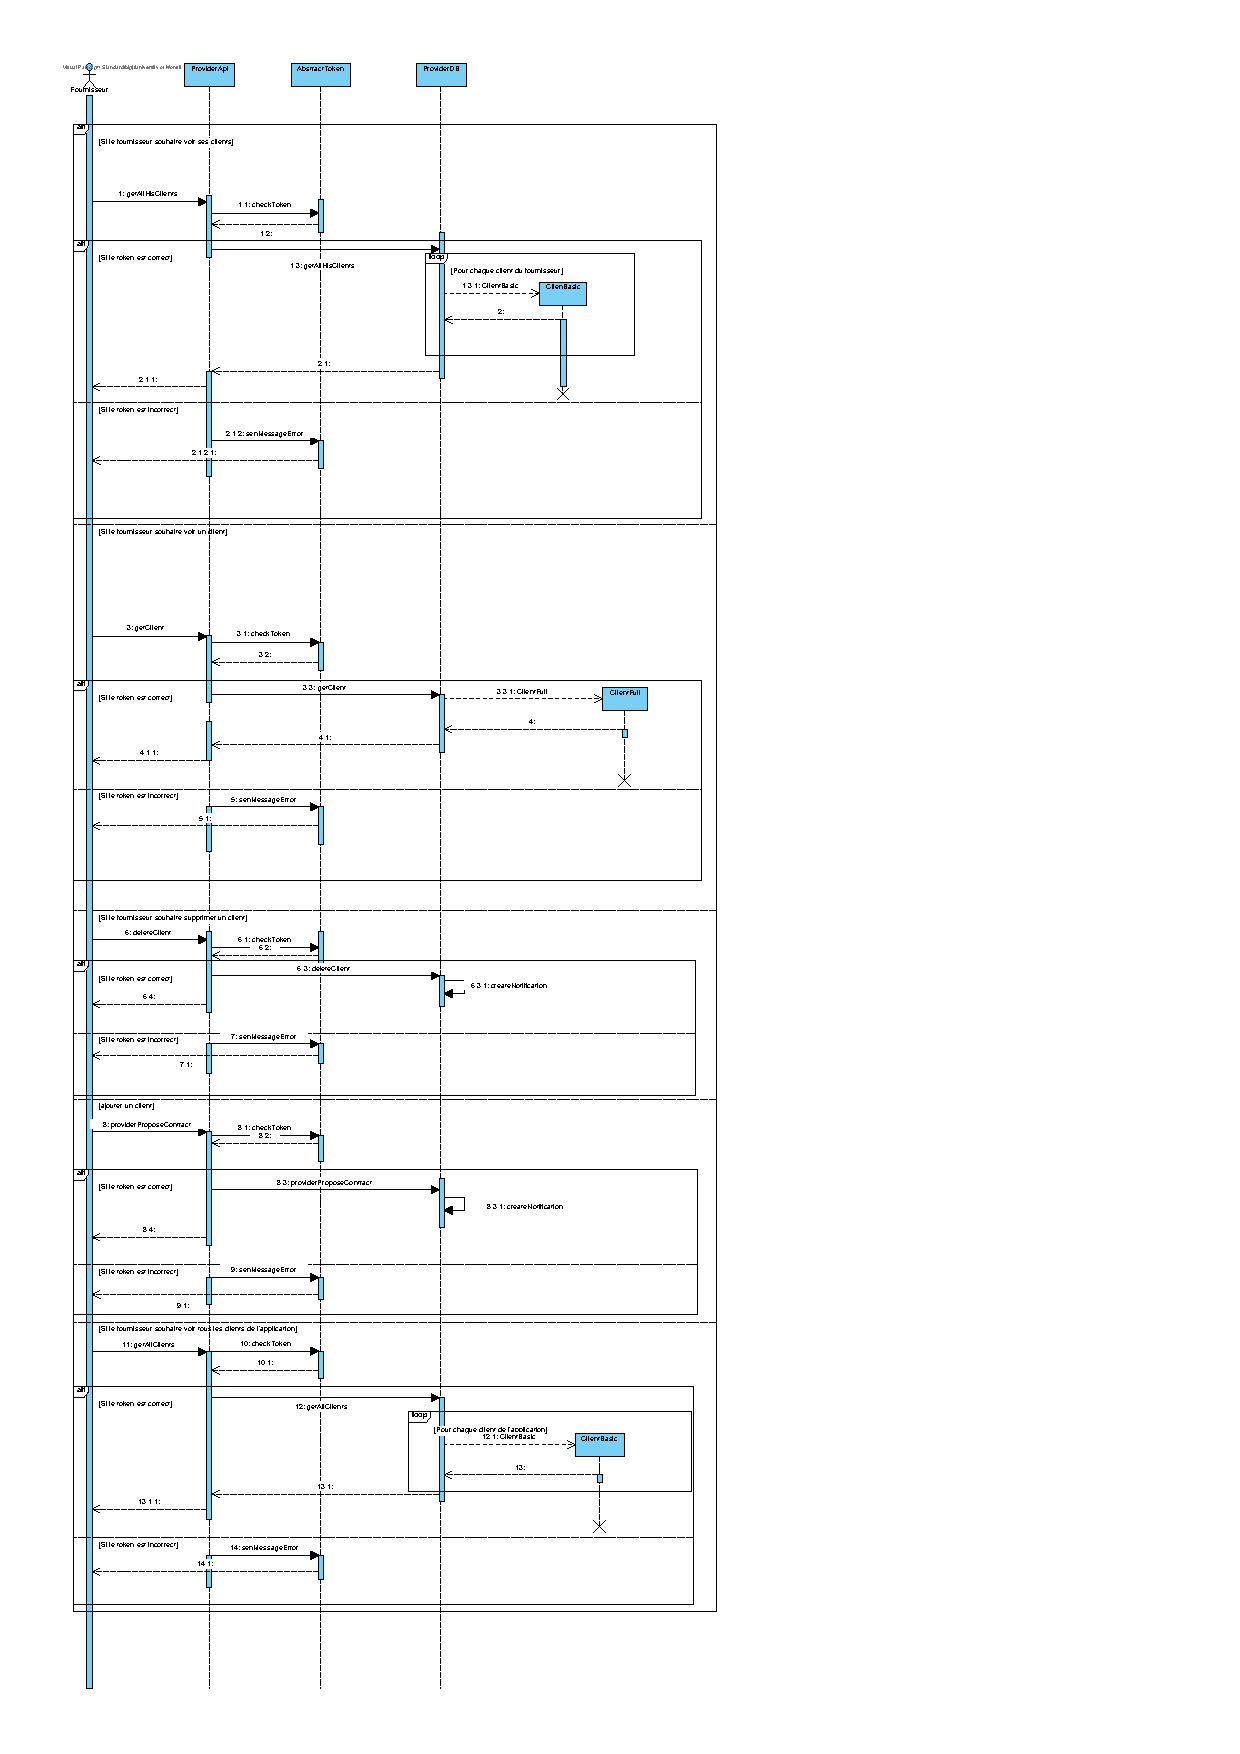
\includegraphics[scale=0.8]{sequence_fournisseur/voir_ses_clients.pdf}
\end{figure}
\newpage
\subsubsection{Gestion des propositions}
\begin{flushleft}
Avant de parler des diagrammes de séquence de cette partie. Nous avons choisis de mettre les contrats d'un fournisseur et ses propositions dans les use cases parlant des contrats. De plus, Seules les propositions seront abordés dans cette partie étant qu'un contrat sera commun au fournisseur et au client(\textit{ie:}  \ref{Common}).
\end{flushleft}

\begin{flushleft}
Pour commencer, nous allons regarder comment le fournisseur peut avoir accès à toutes ses propositions. Pour cela, il devra utiliser la méthode \textbf{getAllProposals}. De plus, une boucle permettra de récupérer tous les objets. Si le fournisseur veut avoir plus de précision sur une de ses propositions, alors il aura juste besoin d'apeller la méthode \textbf{getProposal} en ayant l'identifiant de la proposition au préalable.
\end{flushleft}
\begin{flushleft}
Après ça, Si le fournisseur veut ajouter une proposition. La méthode \textbf{addProposal} sera utilisé. Il faudra néanmoins créer un objet \textbf{ProposalFull} qui sera ensuite ajouté par la précédente méthode à la base de données. 
\end{flushleft}

\begin{flushleft}
Ensuite, si le fournisseur souhaite modifier les paramètres d'une de ses propositions. Il n'aura qu'à faire un nouvel objet qui servira de "remplacant" à l'ancienne proposition. La méthode \textbf{changeProposal} sera appelée par la suite pour faire le changement des paramètres directement dans la base de données. A noter que modifier les paramètres d'une proposition revient à changer les contrats avec les clients qui ont pris cette proposition. De ce fait, une notification sera envoyé via la méthode \textbf{createNotification}.
\end{flushleft}

\begin{flushleft}
Pour finir cette partie, nous allons parler de comment fonctionne la procédure pour supprimer une proposition. Nous avons juste à faire appel à la méthode \textbf{deleteProposal}. De manière similaire au fait de modifier, supprimer implique la supression des contrats des clients ayant comme base cette proposition ce qui implique l'envoie d'une notification par la méthode \textbf{createNotification}.
\end{flushleft}

\begin{figure}[h]
    \centering
    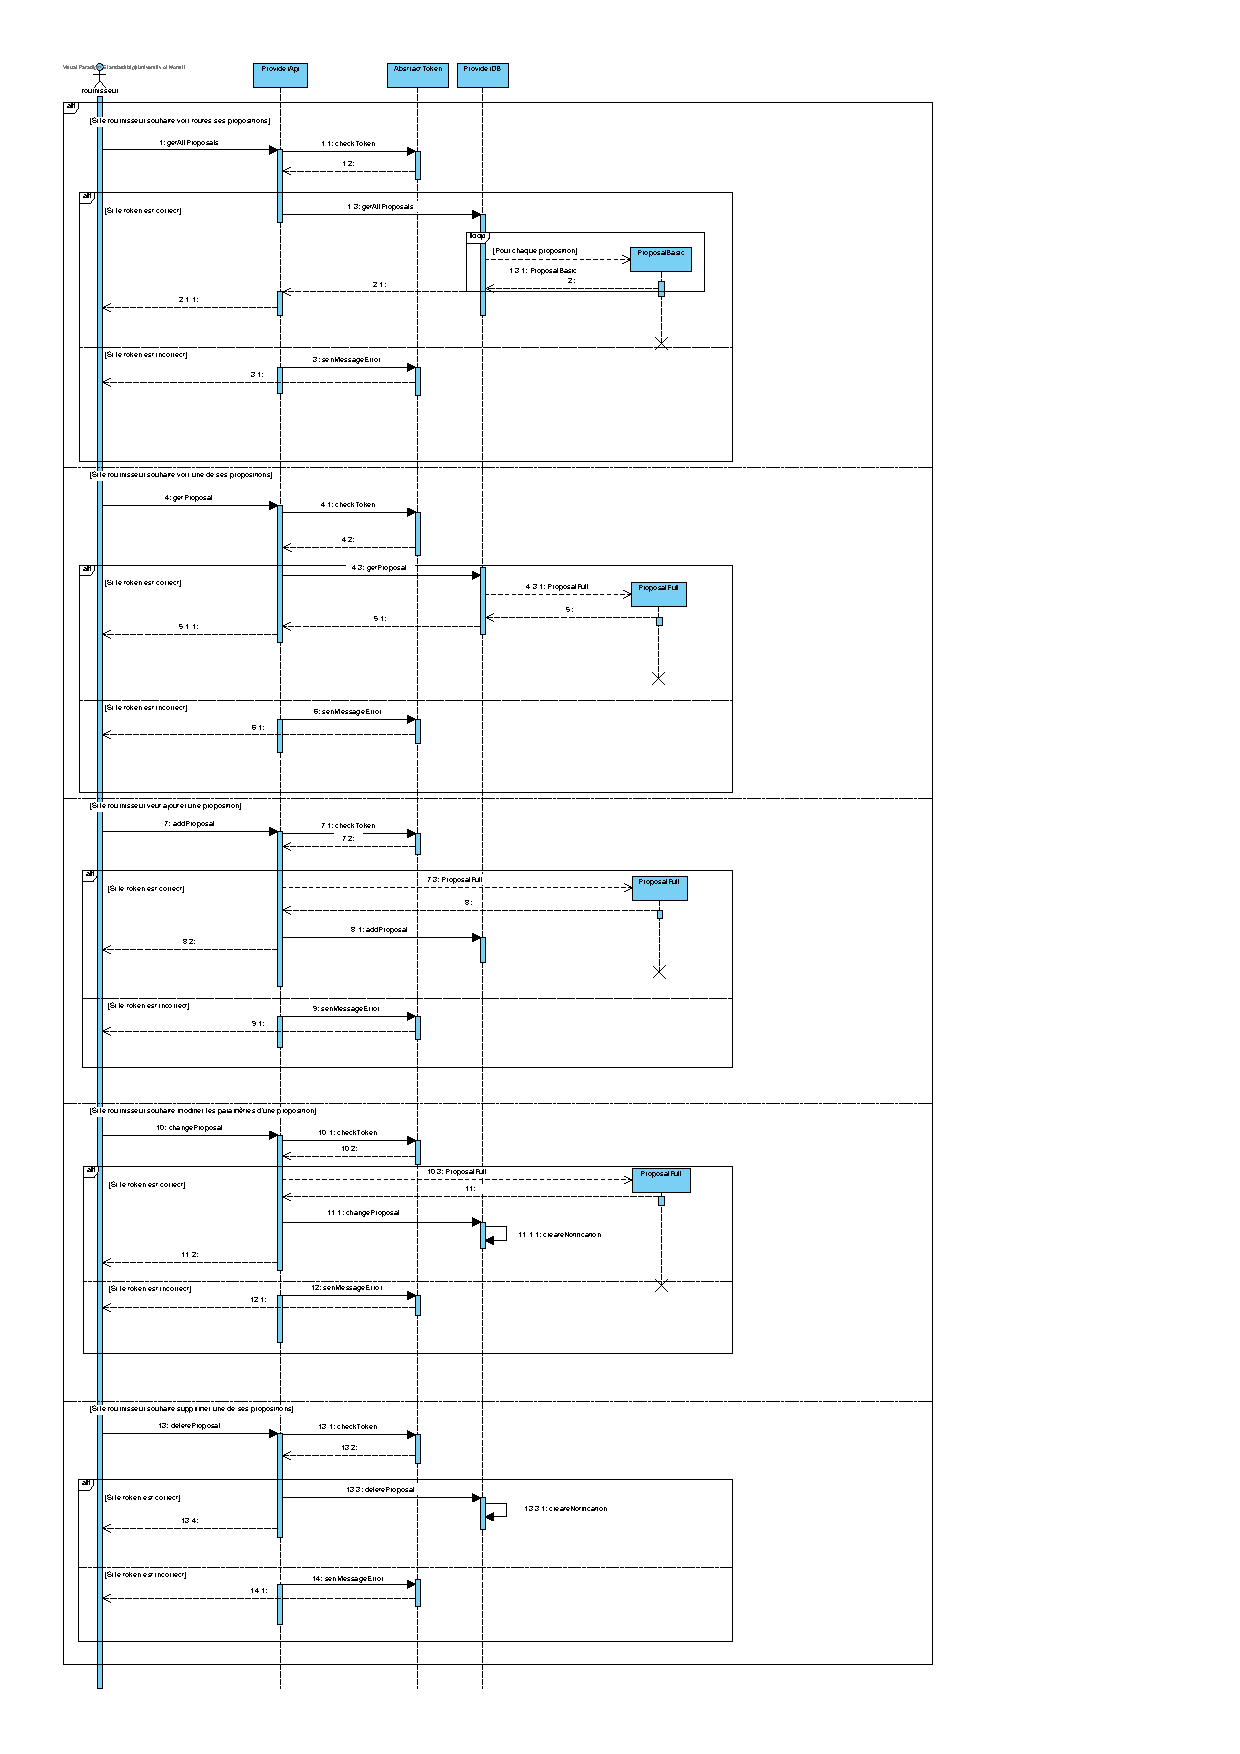
\includegraphics[scale=0.8]{sequence_fournisseur/voir_les_propositions.pdf}
\end{figure}

\newpage
\subsubsection{Gestion de la consommation}
\begin{flushleft}
Cette sous-sous-section parlera de la gestion de la consommation d'un client par le fournisseur. A noter que le fait pour un fournisseur de voir la consommation de ses clients est la même procédure qu'un client qui va voir ses consommations à l'exception qu'un fournisseur ne peut voir la consommation créée par le client liée à son contrat.     
\end{flushleft}

\begin{flushleft}
Tout d'abord, le fournisseur souhaitant supprimer une donnée de consommation devra passer par la méthode \textbf{deleteConsumption} de l'API. En plus de ça, il aura besoin d'un objet date ne contenant que l'année, le mois et le jour. Après ça il pourra supprimer la donnée qu'il souhaite avec la méthode portant le même nom que celle de l'API. Une notification sera envoyé au client avec la méthode \textbf{createNotification}.
\end{flushleft}

\begin{flushleft}
Ensuite, si le fournisseur souhaite supprimer toutes les données de consommation d'un client. Il aura juste besoin de la méthode \textbf{deleteAllConsumption}. De même que le paragraphe du dessus, une notification sera créée.
\end{flushleft}

\begin{figure}[h]
    \centering
    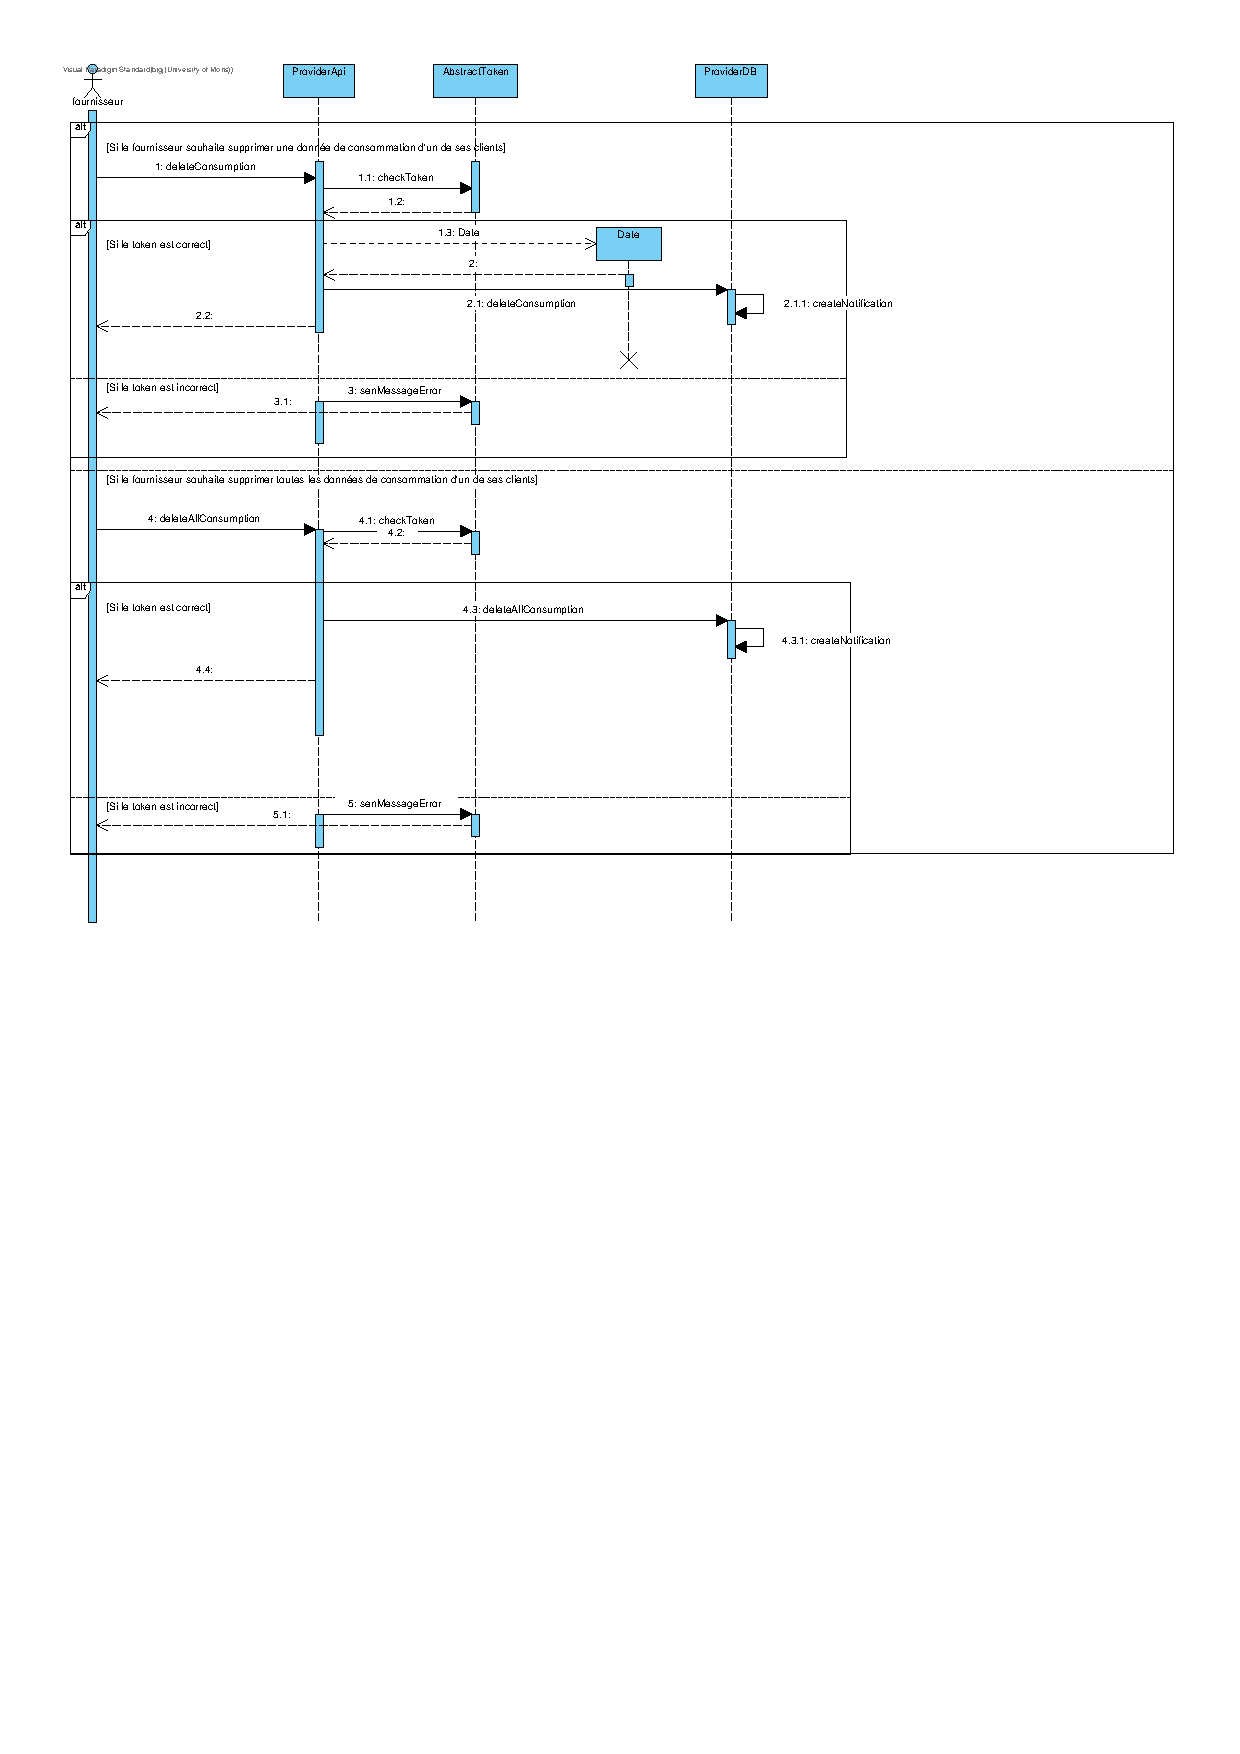
\includegraphics[scale=0.8]{sequence_fournisseur/gestion de la consommation.pdf}
\end{figure}
